%*****************************************
\chapter{Deep Learning and Generative Models}\label{ch:dlgm}
%*****************************************
%Acronym testing: \ac{UML} -- \acs{UML} -- \acf{UML} -- \acp{UML}
\begin{flushright}{\slshape
        By far, the greatest danger of Artificial Intelligence \\
        is that people conclude too early that they understand it.} \\ \medskip
    --- Eliezer Yudkowsky
\end{flushright}

In recent years, \emph{machine learning} techniques have been massively adopted by scientific collaboration around the world. In particular, a paradigm known as \emph{Deep Learning}, which leverages multiple layers of \emph{artificial neurons} trained through the use of a \emph{loss function} and \emph{backpropagation}, has achieved a wide range of applications.

The present chapter will give to the reader a concise but hopefully complete overview of the building blocks behind the recent success of Deep Learning. A splendid introduction, which served the writer well in its own approach to the field, is the one by Michael Nielsen \cite{nielsenneural}. Towards the conclusion we turn to the class of \emph{generative models}, paving the way for the next chapter discussion.
	

\section{Neural Networks}

The name \emph{neural networks} can be understood as a beautiful biologically-inspired programming paradigm, which enables a computer to learn from data. The main idea is (or at least \emph{was}, initially) to simulate how our brains works. In particular, this requires a modelling of the basic brain unit, the neuron, and of its interactions with neighboring units.

\subsection{The Perceptron}

One of the earliest implementation of an algorithm inspired  by our biological brains is due to Rosenblatt \cite{Rosenblatt1958ThePA}. Its \emph{Perceptron} is a type of artificial neuron working exclusively on binary inputs. This scheme mimics the firing of neurons to transmit electrical signals along synapses.

The architecture is illustrated in Figure \ref{fig:rosper}.

\begin{figure}
    \centering
    
    \begin{tikzpicture}
        \node[functions] (left){};
            \node[right = 1.0cm of left] (right) {$y$};
            \path[draw,->] (left) -- (right);
        \node[left=3em of left] (2) {$w_2$} -- (2) node[left of=2] (l2) {$x_2$};
            \path[draw,->] (l2) -- (2);
            \path[draw,->] (2) -- (left);
        \node[below of=2] (dots) {$\vdots$} -- (dots) node[left of=dots] (ldots) {$\vdots$};
        \node[below of=dots] (n) {$w_n$} -- (n) node[left of=n] (ln) {$x_n$};
            \path[draw,->] (ln) -- (n);
            \path[draw,->] (n) -- (left);
        \node[above of=2] (1) {$w_1$} -- (1) node[left of=1] (l1) {$x_1$};
            \path[draw,->] (l1) -- (1);
            \path[draw,->] (1) -- (left);
        \node[above of=1] (0) {$w_0$} -- (0) node[left of=0] (l0) {$1$};
            \path[draw,->] (l0) -- (0);
            \path[draw,->] (0) -- (left);
        \node[above of=l0,font=\scriptsize] {inputs};
        \node[above of=0,font=\scriptsize] {weights};
    \end{tikzpicture}
    
    \caption[The Perceptron]{The Perceptron architecture}
    \label{fig:rosper}
\end{figure}

It has an arbitrary number I of inputs \emph{x$_i$}, to which we associate an equal number of real numbers called \emph{weights w$_i$}. Additionally, we usually add a \emph{bias} term,  which can be seen as adding a \emph{w$_0$} associated with an input constantly set to 1. The neuron outputs a single binary value. The perceptron is a \emph{feedforward} device, meaning that the connections are only from the inputs to the output.

The output $y$ is dictated by a simple algorithmic rule:

\[
\centering
y = 
% f(\pmb{x}) = 
\begin{cases}
1 \quad \text{if} \quad \sum_i w_ix_i + w_0 > 0 \\
0 \quad \text{otherwise}
\end{cases}
\]

where $0$ has been chosen as the \emph{threshold} for the neuron. 
Intuitively, weights measure the importance of the respective inputs to the output, while the bias is a measure of how likely the neuron is to fire. 

Given a set of inputs and their desired outputs, the weights can be tuned (or \emph{learned}) to correctly classify inputs as returning either the $0$ or $1$ outputs. A simple algorithm for doing so is the following:

\begin{outline}[enumerate]
    \1 Initialize the weights. Weights may be initialized to $0$ or to a small random value;
    \1 For each example j in our training set D, perform the following steps over the input $\mathbf {x}_{j}$ and desired output t$_{j}$:
    \2 Calculate the actual output: $y(n)_j = \mathbf{w}\cdot\mathbf{x} + w_0 $
    \2 Update the weights:  $w_{i}(n+1)=w_{i}(n)\;{\boldsymbol {+}}\;r\cdot (t_{j}-y_{j}(n))x_{j,i}$
    \1 The second step may be repeated until the iteration error \\
    $\frac{1}{s} \sum_{j=1}^{s}|t_{j}-y_{j}(n)|$ is less than a user-specified error threshold $\gamma$, or a predetermined number of iterations have been completed.
\end{outline}

This first example of \emph{learning algorithms} is showing how we can actually use artificial neurons in a way which is radically different to conventional logic gates. Instead of explicitly laying out a circuit of NAND and other gates, our neural networks can simply learn to solve problems, sometimes problems where it would be extremely difficult to directly design a conventional circuit.

Despite this, the single Perceptron presents several limitations. Ultimately, it is a \emph{linear classifier}, meaning that:

\begin{outline}
    \1 It cannot solve a problem if it is not \emph{linearly separable}, so for example even a simple XOR division of the binary plane is unsolvable;
    \1 It is only capable of addressing classification problems, and cannot tackle our generation task.
\end{outline}

Nonetheless, the simple ideas behind this architecture are actually at the heart of the more modern and refined approach of deep learning.

\subsection{Neural Networks and Backpropagation}

Turning back once more to our biological brain, we can observe that it is actually made up by \emph{billions} of neurons. Intuitively, we would expect that an artificial network made up of multiple artificial neurons would demonstrate better capacities than a single neuron--and unsurprisingly that's how it is. 

Figure \ref{fig:firstnn} shows a first example of a proper feedforward neural \emph{network}: an ensemble of neurons organized in \emph{layers}, where each layer is \emph{fully connected} to the neurons in the previous one. One early result, sparking the interest in the field, showed that a neural network with just \emph{one} hidden layer with a large enough number of neurons can approximate any arbitrary function \emph{f} \cite{HORNIK1989359}.

\begin{figure}
    \centering
    \begin{neuralnetwork}[height=4]
        \newcommand{\x}[2]{$x_#2$}
        \newcommand{\y}[2]{$\hat{y}_#2$}
        \newcommand{\hfirst}[2]{\small $h^{(1)}_#2$}
        \newcommand{\hsecond}[2]{\small $h^{(2)}_#2$}
        \inputlayer[count=3, bias=true, title=Input\\layer, text=\x]
        \hiddenlayer[count=4, bias=false, title=Hidden\\layer $1$, text=\hfirst] \linklayers
        \hiddenlayer[count=3, bias=false, title=Hidden\\layer $2$, text=\hsecond] \linklayers
        \outputlayer[count=2, title=Output\\layer, text=\y] \linklayers
    \end{neuralnetwork}
    \caption[A simple neural network]{A simple neural network architecture with two \emph{hidden} layers.}
    \label{fig:firstnn}
\end{figure}

Intuitively, this architecture is taking advantage of its various neurons by letting the first hidden layer process the input data, and then allowing subsequent layers to act on the previous outputs. The relevant information gets extracted from the high level features in the input data, and the network allows only the important bits to travel further down in the architecture. 

But if the single neuron was modelled as the Perceptron, the outputs would be only $0$s and $1$s--not that different from the actual binary inputs. Besides, we would also like to move away from the binary-inputs-only limitation. With just a few tweaks to the original Perceptron architecture, we may obtain something more general and more well suited to our new architecture.

\paragraph{Neurons and activation functions}

First of all, we allow for continuous inputs. Then, we would like to employ a neuron with the following property: \emph{a small change in the \emph{weights} or \emph{biases} causes a small change in the \emph{outputs}}. This seems reasonable to allow the overall network to learn by gradually adjusting its parameters, and may also be translated in more physical terms by the following expression:

\begin{equation}\label{eqn:yderiv}
  \Delta y = \sum_j \frac{\delta y}{\delta w_j}\Delta w_j + \frac{\delta y}{\delta w_0}\Delta w_0
\end{equation}



where we have introduced the partial derivatives over the weights and the bias.

It is clear that the Perceptron does not respect this property, since an arbitrary small change could cause an abrupt shift in the output from $0$ to $1$ or vice-versa. This issue is easily resolved by adding an \emph{activation function} to the output, as shown in Figure \ref{fig:artneur}.

\begin{figure}
    \centering
    
    \begin{tikzpicture}
        \node[functions] (left){};
            \node[right = 1.0cm of left] (right) {$y=f(\mathbf{w}\cdot\mathbf{x} + w_0)$};
            %\node[right of = right] (rright) {$=f(\mathbf{w}\cdot\mathbf{x} + w_0)$};
            \path[draw,->] (left) -- (right);
        \node[left=3em of left] (2) {$w_2$} -- (2) node[left of=2] (l2) {$x_2$};
            \path[draw,->] (l2) -- (2);
            \path[draw,->] (2) -- (left);
        \node[below of=2] (dots) {$\vdots$} -- (dots) node[left of=dots] (ldots) {$\vdots$};
        \node[below of=dots] (n) {$w_n$} -- (n) node[left of=n] (ln) {$x_n$};
            \path[draw,->] (ln) -- (n);
            \path[draw,->] (n) -- (left);
        \node[above of=2] (1) {$w_1$} -- (1) node[left of=1] (l1) {$x_1$};
            \path[draw,->] (l1) -- (1);
            \path[draw,->] (1) -- (left);
        \node[above of=1] (0) {$w_0$} -- (0) node[left of=0] (l0) {$1$};
            \path[draw,->] (l0) -- (0);
            \path[draw,->] (0) -- (left);
        \node[above of=l0,font=\scriptsize] {inputs};
        \node[above of=0,font=\scriptsize] {weights};
    \end{tikzpicture}
    
    \caption[Generic artificial neuron]{A more generic architecture for the artificial neuron, leveraging an activation function \emph{f}.}
    \label{fig:artneur}
\end{figure}

The particular choice of activation function defines the type of the neuron. The key characteristic is that the activation function should be \emph{differentiable}, to allow the computation of \eqref{eqn:yderiv}. Many possible choices have been explored and proposed in past years.
\graffito{Note: The Perceptron can be seen as a generic neuron with the activation function set to the step function in $0$.}
Historically, the \emph{Sigmoid} function has been the most popular choice:

\[
y=f(\mathbf{w}\cdot\mathbf{x} + w_0) = \frac{1}{1 + e^{-\mathbf{w}\cdot\mathbf{x} - w_0}}
\]

which has the nice property of presenting a smooth transition between the two saturating extremes of the Perceptron, as well as having a derivative which can be easily re-expressed in term of the Sigmoid itself. Nowadays, the \emph{Rectified Linear Unit} (ReLU) function has demonstrated better capabilities, especially in large and complex networks:

\[
y=f(\mathbf{w}\cdot\mathbf{x} + w_0) = 
\begin{cases}
\mathbf{w}\cdot\mathbf{x} + w_0 \quad \text{if} \quad \mathbf{w}\cdot\mathbf{x} + w_0 > 0 \\
0 \quad \text{otherwise}
\end{cases}
\]

despite not being analytically differentiable in $0$ (it is standard practice to set the derivative in the point to $0$). Figure \ref{fig:actfunc} shows a comparison between the two.

\begin{figure}
    \centering
    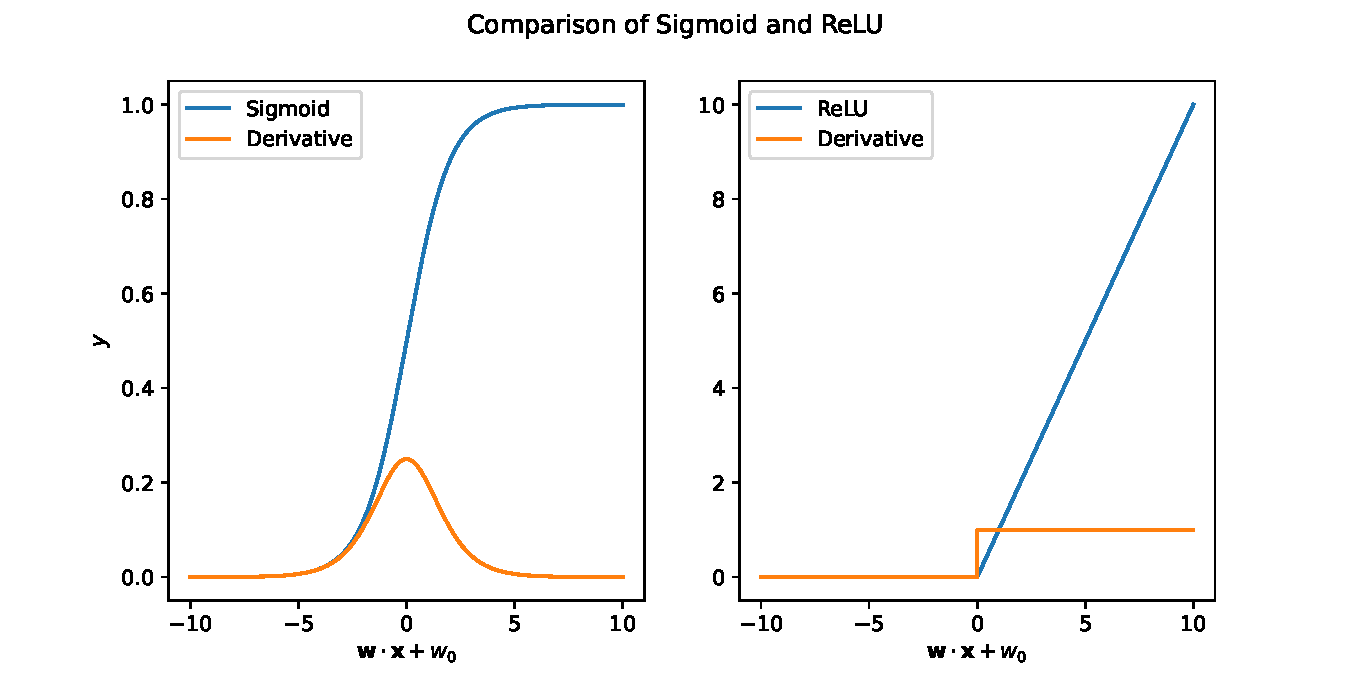
\includegraphics[scale=0.50]{gfx/ch2/activ.pdf}
    \caption[Activation functions]{The Sigmoid activation function compared to the ReLU, along with the respective derivatives w.r.t. the full input vector.}
    \label{fig:actfunc}
\end{figure}

We will discuss other useful properties of the ReLu function in the following.

\paragraph{Gradient descent and backpropagation}

Now that we have devised a well suited neuron for the architecture of Figure \ref{fig:firstnn}, the objective is straightforward: \emph{find the optimal set of \emph{model parameters} (the weights) for solving the current problem.} 

Typically an \emph{objective function} or \emph{loss function} is defined, as a function
of $\mathbf{w}$, to measure how well the network with weights set to $\mathbf{w}$ solves the task. 
The objective function is a sum of terms, one for each input/target pair ($\mathbf{x}$, $\mathbf{t}$),
measuring how close the output $y$($\mathbf{x}$, $\mathbf{t}$) is to the target $\mathbf{t}$. We can denote it with $\mathcal{L}$($\mathbf{x}$, $\mathbf{t}$).

The training process is an exercise in \emph{function minimization} – i.e., adjusting $\mathbf{w}$ in such a way as to find a $\mathbf{w}$ that minimizes the objective function. Our physical intuition suggests that this might have something to do with the \emph{gradients} of the loss function. As we have already discussed, we can write the following relationship:

\[
    \Delta \mathcal{L} = \frac{\delta \mathcal{L}}{\delta \mathbf{w}} \cdot \Delta \mathbf{w} = \nabla_w \mathcal{L} \cdot \Delta \mathbf{w} 
\]
 where we have introduced the \emph{gradients vector} $\nabla_w \mathcal{L}$. If we now change the parameters at each step by an amount $ \Delta \mathbf{w} = - \eta \nabla_w \mathcal{L}$, where $\eta$ is an hyperparameter called \emph{learning rate}, we will get a corresponding change in the loss function of:
 
 \[
    \Delta \mathcal{L} = -\eta \nabla_w \mathcal{L} \cdot \nabla_w \mathcal{L} = - \eta \|  \nabla_w \mathcal{L} \|^2
\]

that is, we have updated the parameters in a way which is reducing the loss, meaning that the outputs of our network are actually getting closer to our targets--i.e. the network is \emph{learning} the optimal parameters directly from the training data! This is the idea behind \emph{gradient descent} learning algorithms, which are the current standard for training deep neural networks. The main steps are as follows:

\begin{outline}[enumerate]
    \1 Select a \emph{batch} of input/target pairs ($\mathbf{x}$, $\mathbf{t}$)$^n$ and compute the outputs y$^n$ = \emph{f}($\mathbf{x}$, $\mathbf{t}$)$^n$;
    \1 Compute $\mathcal{L}$($y^n$), $\nabla_w \mathcal{L}^n$ and find $ \Delta \mathbf{w}^n = - \eta \nabla_w \mathcal{L}^n$;
    \1 For each batch, update the weights as $ \Delta \mathbf{w} = - \eta \sum_n \nabla_w \mathcal{L}^n$
\end{outline}

where we are assuming that the loss function may be expressed as an average of over cost functions for individual training examples. The dataset is processed multiple times as finite batches until the network reach some sort of global minimum for the loss function.

The only non trivial thing which remains to do is define the best way to compute $\nabla_w \mathcal{L}$. This can be done efficiently, with just one forward and one backward pass through the network, through the \emph{backpropagation} algorithm.


\subsection{Deep Learning}
% also mention problems?
% mention residual networks?
\section{Generative Models}

\subsection{State of the art}

\subsection{Known issues}
% low dim paper?

%*****************************************
%*****************************************
%*****************************************
%*****************************************
%*****************************************
